\chapter{Literature Review}\label{literature}

In this chapter, the first existing inverter modeling approaches are presented, and then the candidate model, i.e., eigenvalue-based literature, is elaborated on in more detail.
\section{Power System Phenomena Classification}
\begin{figure}[ht]
    \centering
	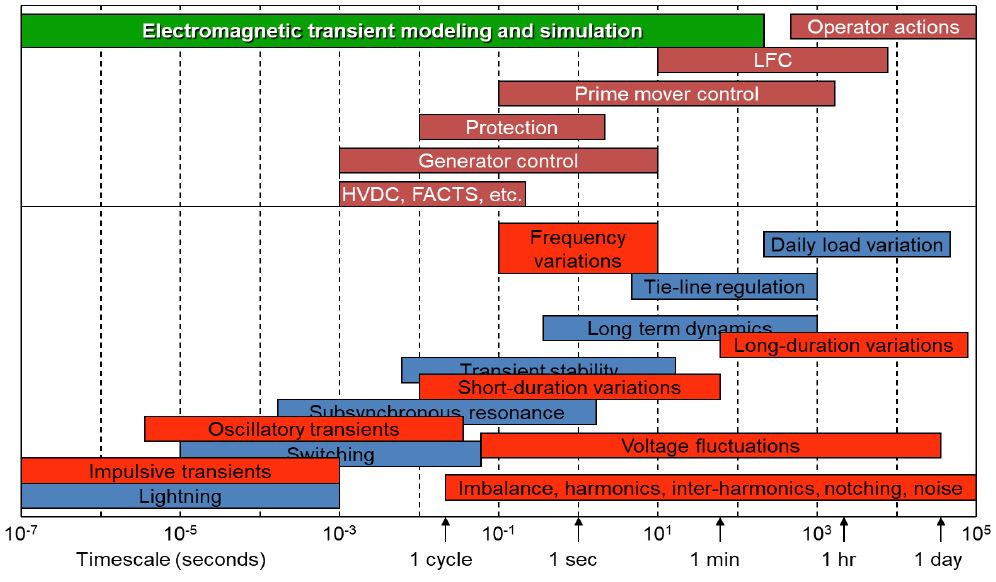
\includegraphics[width=0.85\textwidth]{figures/Picture1.jpg}
	\caption[Power system phenomena]{Power system phenomena and required accuracy of modeling.\cite{PSCAD}}
	\label{fig:ph}
\end{figure}

\ref{fig:ph} shows the different power system phenomena and their time scales. In power system modeling and study it is very important to chose a time scale that captures the desired phenomena and meanwhile is computationally efficient. Two main types of power system modeling are \gls{EMT} and \gls{RMS}. Other modeling approaches are categorized within one of the aforementioned modeling methods.

\section{\gls{EMT}-Based Model}

\subsection{Dommel's Method}
 EMT model, the most exact model of an electrical device, considers time domain differential equations of all circuit elements and solves them in the time domain. The first computationally feasible approach was introduced by Domell in the late 60s \cite{EMT1} \cite{EMT2}. In Dommel's method, every linear and nonlinear circuit element is modeled as a current source in parallel with a linear circuit element within a specific time interval. Dommel's method is still being used in software tools such as PSCAD (EMTDC) and EMTP. These methods are computationally time-consuming and must be used when a very high-frequency phenomenon needs to be captured or when the maximum short circuit current caused by a high-frequency component in the waveform needs to be measured. 

\subsection{Piece-wise Average Model}
One of the significant causes of nonlinearity in power system components is semiconductor devices that exist in all inverters. Including the exact model of these switches makes simulation time enormously long. To accelerate EMT simulations of the PWM converters, a novel algorithm was proposed later, which integrates an improved averaged model of \gls{PWM} inverters into the \gls{EMT}. \cite{ImprovedAvg} The performance of this method is acceptable in studying specific switching and short circuits that include \gls{PWM} inverters. However, this average model integration makes the simulation inaccurate for faster phenomena such as lightnings. 

\subsection{Dynamic Phasor Modeling}
Dynamic phasors are also another method that tries to make a bridge between \gls{EMT} and \gls{RMS} methods. For example, a dynamic phasor model of a \gls{MMC} with extended
the frequency range for direct interfacing to an EMT simulator is introduced in \cite{DP} and \cite{DP2}. The internal dynamics of the \gls{MMC}
are modeled considering dominant harmonic components of
each variable. To model the external dynamics of the converter,
a novel construct referred to as a base-frequency is employed,
which allows to capture and model any number of frequency
components of external variables without any significant increase in
computational burden \cite{DP}.


\section{\gls{RMS}-Based Models}

Because the slower phenomena can be accurately captured with a less complicated method, using time-consuming EMT modeling for every phenomenon seems unnecessary. Therefore, methods such as \gls{RMS} with lesser computational burdens are developed to tackle the speed problem. \gls{RMS} models are models that use the phasor model of components and are lighter than EMT models. \gls{RMS} models are widely used in software tools such as MATLAB Simulink and DIgSILENT Powerfactory. This modeling approach is a basis for some inverter models, as follows:

\subsection{Average Model}

The average model linearizes the inverter switching by considering an average value of two on and off cycles. \cite{AVG} This approximation enables \gls{RMS} to include inverters in the simulation. The average model is widely used in inverter design, stability, and control and is a basis for other inverter \gls{RMS} models.  

\subsection{Generic Models}

Generic models comes as a package and include most of control block diagrams and circuit components for inverters. Generic models are developed by standards in order to make a general widely used model of inverters, so that can be used as benchmark in industry and academia. For example Generic models of \gls{WECC} are presented and validated for wind and solar energy integration \cite{GenericWECC}. These models have their own limitations and flexibility problems and may not be suitable for particular phenomena or particular inverter functionality. In addition, because standards provide them, they are being updated slowly, and new technologies cannot be implemented readily in generic models.

\subsection{Eigenvalue Based}

In order to capture certain power system phenomena such as inter-area oscillations and ensure small-signal stability in conventional systems, eigenvalue analysis is a well-established method \cite{kundur}. However, implementing this method for inverter-based systems is a novel concept. In \cite{invertermodal} a modal analysis is made for a coupled \gls{GFM} and \gls{GFL} using a global eigenvalue analysis. The results are accurate for a two-inverter system, but the method lacks modularity and scalability. Unified impedance models, however, solve this problem. In \cite{hr} and \cite{Uni}, the complex transfer function formulation, which is the benchmark of small-signal studies, is introduced. A complete model is later introduced in \cite{Uni} In \cite{Bwen}, an additional $dq/abc$ transform block is added to the small-signal model. Finally, in \cite{scholes2011lessons}, a small-signal model for \gls{GFM} is introduced, which is limited to the \gls{VIL} GFMs. Therefore, an analysis of the other GFM topologies alongside with GFLs is still unexamined. Besides, in the literature mentioned, GFMs are considered a constant angle device, and the GFM angle generation loop is not considered. 

\section{Section Summary}

This chapter provided a literature review on the modeling of inverters. Among different methods, eigenvalue (small-signal) based methods built based on the average switch model are more suitable for inter-area oscillation studies. Besides the valuable literature on the inverter small-signal concept, the small-signal model is the most efficient method for studying oscillations for different inverter GFM topologies. Steady-state angle difference, DC side dynamics, and LCL filter effect are not considered holistically. In this thesis, the focus is to include different inverter strategies and also include all possible block diagrams comprehensively. Later, the explicit small-signal parametric equations are derived numerically to be used in a scalable approach.


